%********************************************************************
% Appendix
%*******************************************************
% If problems with the headers: get headings in appendix etc. right
%\markboth{\spacedlowsmallcaps{Appendix}}{\spacedlowsmallcaps{Appendix}}
\chapter[Expérience annexe: période d'attention]{Séquence d'événements ou texture sonore: l'influence de la période d'attention.}
\label{app:xp_texture}

\gl{TODO: ajout des autres expériences}

\section{Objectif de l'expérience}

Nous présentons ici les résultats d'une étude sur la perception des textures sonores, étude menée dans le cadre de cette thèse, mais déconnectée du sujet principal. 

Comme nous l'avons vu (\cf~Section~\ref{sec:ch3_textureDef}), la texture est un objet composite, dont les éléments constitutifs cessent d'être perçus de manière distinctes, dès lors qu'ils occurrent suivant un pattern dont les caractéristiques physiques restent stables au cours du temps. La perception de ce pattern nécessite une certaine période d'attention. C'est cette période que nous nous proposons d'étudier.

En poussant la vision composite d'une texture à l’extrême, nous considérons qu'une texture peut être vue comme un empilement d'événements sonores, si tant est que la séquence de ces événements forme un tout homogène au sens des textures (\cf~Section~\ref{sec:ch3_textureDiscussion}). 

Nous suivons cette idée, et proposons un protocole expérimentale permettant d'analyser la période d'attention. 

En considérant comme stimuli une mixture d'événements du même type, nous faisons l'hypothèse qu'à partir du moment où le cerveau parvient à isoler un événement de cette mixture, il ne perçoit plus la mixture comme une texture, mais comme une succession d'événements. Inversement, s'il ne parvient pas à distinguer un événement isolé, alors la mixture est perçue comme une texture.

Nous appliquons le modèle de scène sonore proposé (\cf~Section~\ref{sec:ch4_modelForm}) afin de simuler des textures à partir de séquences d'événements dont nous contrôlons l'espacement \emph{inter-onsets} moyen. Il s'agit de faire varier cet espacement, afin d’identifier le seuil à partir duquel la séquence d'événements cesse d'être perçue comme une texture. 

À ce titre, le protocole proposé s'inscrit complètement dans le cadre des expériences perceptives portant sur la détection du signal. La section~\ref{app:sdt} présentent de manière résumée les spécificités méthodologiques et les hypothèses sur lesquels s'appuient ces expériences de détection.

\section{Banque de données}

Chaque stimuli est composé d'un son cible, suivi d'une séquence d'événements enchevêtrés. Tous les événements sont des sons isolés ayant une durée de $1$ seconde. La séquence dure 6 secondes. L'objectif pour le sujet est d'indiquer si oui ou non il a entendu le son cible dans la séquence d’événements. 

Les séquences donnent à entendre des scènes de trafic. Ces scènes sont simulées en agglomérant des sons de voiture isolés. La simulation est contrôlée par un paramètre réglant l'espacement temporel \emph{inter-onsets} moyen entre les événements. Cinq valeurs d'espacement sont considérées: $0.1$, $0.3$, $0.5$, $0.7$ et $0.9$ secondes (\cf~Figure~\ref{fig:xptexturea}, et~\ref{fig:xptextureb}). 

Pour chaque espacement, nous simulons 20 séquences de trafics, chaque sujet devant alors écouter 100 stimuli. La moitié de ces stimuli sont des pièges (\emph{catch trial}), le son cible y étant absent.

Le son cible est le même pour tous les stimuli et tous les sujets. Il a été choisi par les expérimentateurs, afin d'être d'être à mi chemin entre un son très identifiable, et un son dénué de caractéristiques saillantes.

\section{La théorie de la détection du signal}
\label{app:sdt}

\section{Planification expérimentale}

\subsection{Procédure}

L'expérience une épreuve d'évaluation de type oui/non (\cf~Section~\ref{app:sdt}). Chaque sujet évalue l'ensemble des 100 stimuli. Pour chaque stimulus, il doit répondre si oui ou non il a entendu le son cible.

Pour chaque sujet, les scènes sont présentées dans un ordre aléatoire. 

\subsection{Apparatus}

Tous les sujets passent l'expérience sur des machines identiques \gl{description des machines}. L'audio est diffusé en monophonique, par le biais de casques audio semi-ouvert \emph{Beyer-Dynamic DT 990 Pro}. 

Le niveau sonore de sortie est le même pour tous les sujets. Il a été préalablement fixé par les expérimentateurs afin de correspondre à un niveau d'écoute confortable.

Les sujets passent l'expérience individuellement, dans un environnement acoustique calme. Un expérimentateur est présent durant la totalité de l'expérience, afin de contrôler le bon déroulement de cette dernière, et de répondre aux éventuelles questions des sujets.

\subsection{Participants}


\section{Méthodologie et outils statistiques}

\gl{TODO: indiquer $d'>1$}.

Nous mesurons les performances des sujets en utilisant la mesure de sensitivité $d'$ (\cf~Section~\ref{app:sdt}).
 
\section{Résultats}

\begin{figure}[t]
        \myfloatalign
        \subfloat[]
        {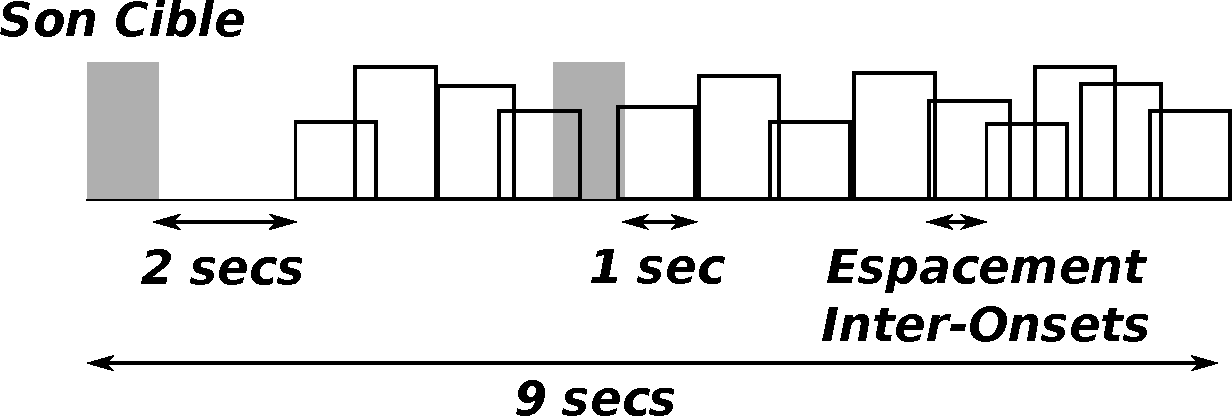
\includegraphics[width=.5\linewidth]{gfx/xpTexture1}\label{fig:xptexturea}}
        \subfloat[]
        {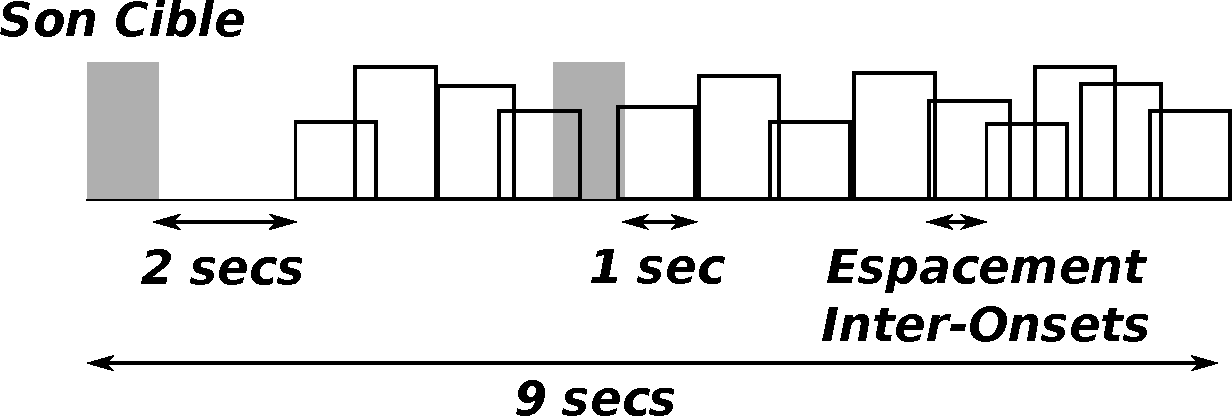
\includegraphics[width=.5\linewidth]{gfx/xpTexture1}\label{fig:xptextureb}} \par
        \subfloat[]
        {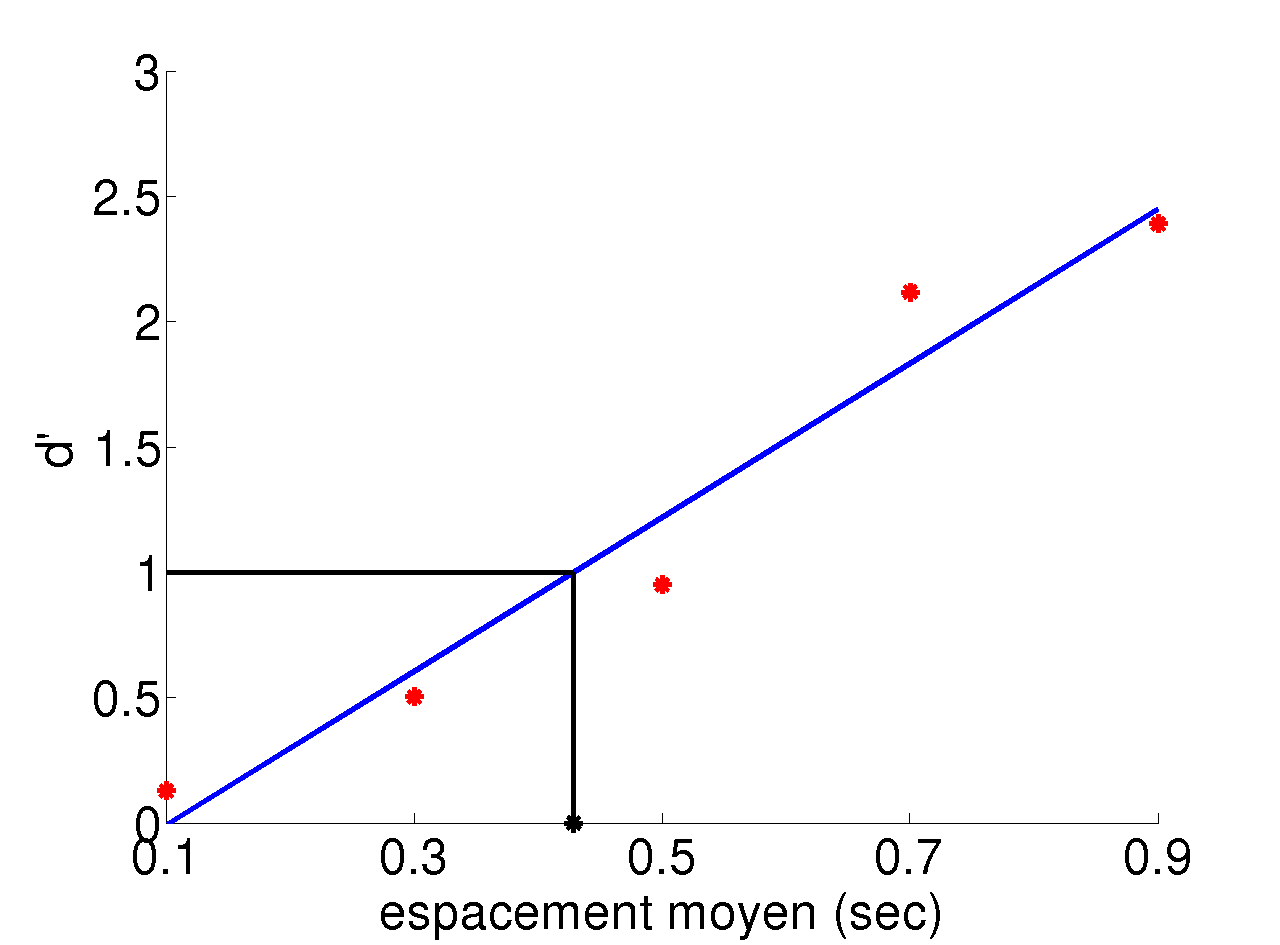
\includegraphics[width=.5\linewidth]{gfx/xpTexture3}\label{fig:xptexturec}}
        \caption[Événement ou texture sonore: influence de la période d'attention]{Événement ou texture sonore: influence de la période d'attention. (a) stimulus un ayant un espacement temporelle faible \gl{TODO}; (b) stimulus un ayant un espacement temporelle élevé \gl{TODO}; (c) le seuil d'espacement moyen permettant de faire la distinction entre une séquence d'événements et une texture }\label{fig:xptexture}
\end{figure}

\gl{TODO}.

Les résultats sont très encourageants. Ils montrent qu'il existe bien un espacement limite à partir duquel la mixture cesse d'être perçue comme une texture (\cf~Figure~\ref{fig:xptexturec}). Pour des sons isolés d'une seconde, cet espacement limite est de 0.42 secondes, soit la moitié de la durée des événements utilisés.

 


